\documentclass[12pt]{article}\usepackage{graphicx, color}
\usepackage{alltt}
\usepackage[left=1in,top=1in,right=1in,bottom=1in,nohead]{geometry}
\usepackage{geometry}                % See geometry.pdf to learn the layout options. There are lots.
\geometry{a4paper}                   % ... or a4paper or a5paper or ... 
\usepackage{wrapfig}	%in-line figures
\usepackage[square, comma, sort&compress]{natbib}		%bibliography
\usepackage{pslatex} 	%for times new roman
\usepackage[parfill]{parskip}    % Activate to begin paragraphs with an empty line rather than an indent
\usepackage{graphicx}
\usepackage{amssymb}
\usepackage{epstopdf}
\usepackage{booktabs}
\usepackage{amsmath}
\usepackage{color} % for coloring of text
\usepackage[usenames,dvipsnames]{xcolor} % More colors
\usepackage{multirow}
\usepackage{outlines}
\usepackage{xfrac}
\usepackage{relsize} % for scaling parts of equations. e.g. \mathlarger
\usepackage{hyperref}
\usepackage{rotating}
\usepackage{array} 

\linespread{1} %remove for double space

\DeclareGraphicsRule{.tif}{png}{.png}{`convert #1 `dirname #1`/`basename #1 .tif`.png}

\providecommand{\e}[1]{\ensuremath{\times 10^{#1}}}

\makeatletter
\newcommand{\thickhline}{%
    \noalign {\ifnum 0=`}\fi \hrule height 1pt
    \futurelet \reserved@a \@xhline
}

\begin{document}

\newcommand{\multilineR}[1]{\begin{tabular}[b]{@{}r@{}}#1\end{tabular}}
\newcommand{\multilineL}[1]{\begin{tabular}[b]{@{}l@{}}#1\end{tabular}}
\newcommand{\multilineC}[1]{\begin{tabular}[b]{@{}c@{}}#1\end{tabular}}

\section*{Supplemental figure summary}

\begin{outline}
\1 F\ref{fig:boundFlux}: boundary fluxes
\1 F\ref{fig:fluxHM}: fluxHM
\1 F\ref{fig:proteomicsConsistency}: protein fold change reproducibility
\1 F\ref{fig:proteinHM}: proteinHM
%\1 F\ref{fig:TPMomics}: impact of GR and limitation on abundance
\1 T\ref{protTable}: proteomics enzyme coverage
%\1 F\ref{fig:enzymeHM}: enzyme HM
\1 T\ref{tab:GS}: summary of well-supported regulation
\1 F\ref{fig:atpprtase}: ATP-PRTase in vitro biochemistry
\1 F\ref{fig:otcase}: OTCase in vitro biochemistry
\1 F\ref{fig:hypoMet}: Using optimal regulators to investigate the regulation of understudied reactions
\1 T\ref{tab:all_rxn}: table of supported regulation for each reaction
\1 F\ref{fig:occupancy} occupancy comparison
\1 F\ref{fig:paramaterValues}: thermodynamic comparison
%\1 F\ref{fig:dahp}: DAHP synthase
%\1 SF7: reversibilityImprovement
\1 F\ref{fig:MLbar}: metabolic leverage bar
\1 F\ref{fig:MLpathways}: coloring amino acid and nucleotide pathways based on ML
\1 F\ref{fig:MCA}: MCA model of glycolysis

\end{outline}

\newpage

\makeatletter 
\renewcommand{\thefigure}{S\@arabic\c@figure}
\renewcommand{\thetable}{S\@arabic\c@table}
\makeatother

\begin{figure}[h!]
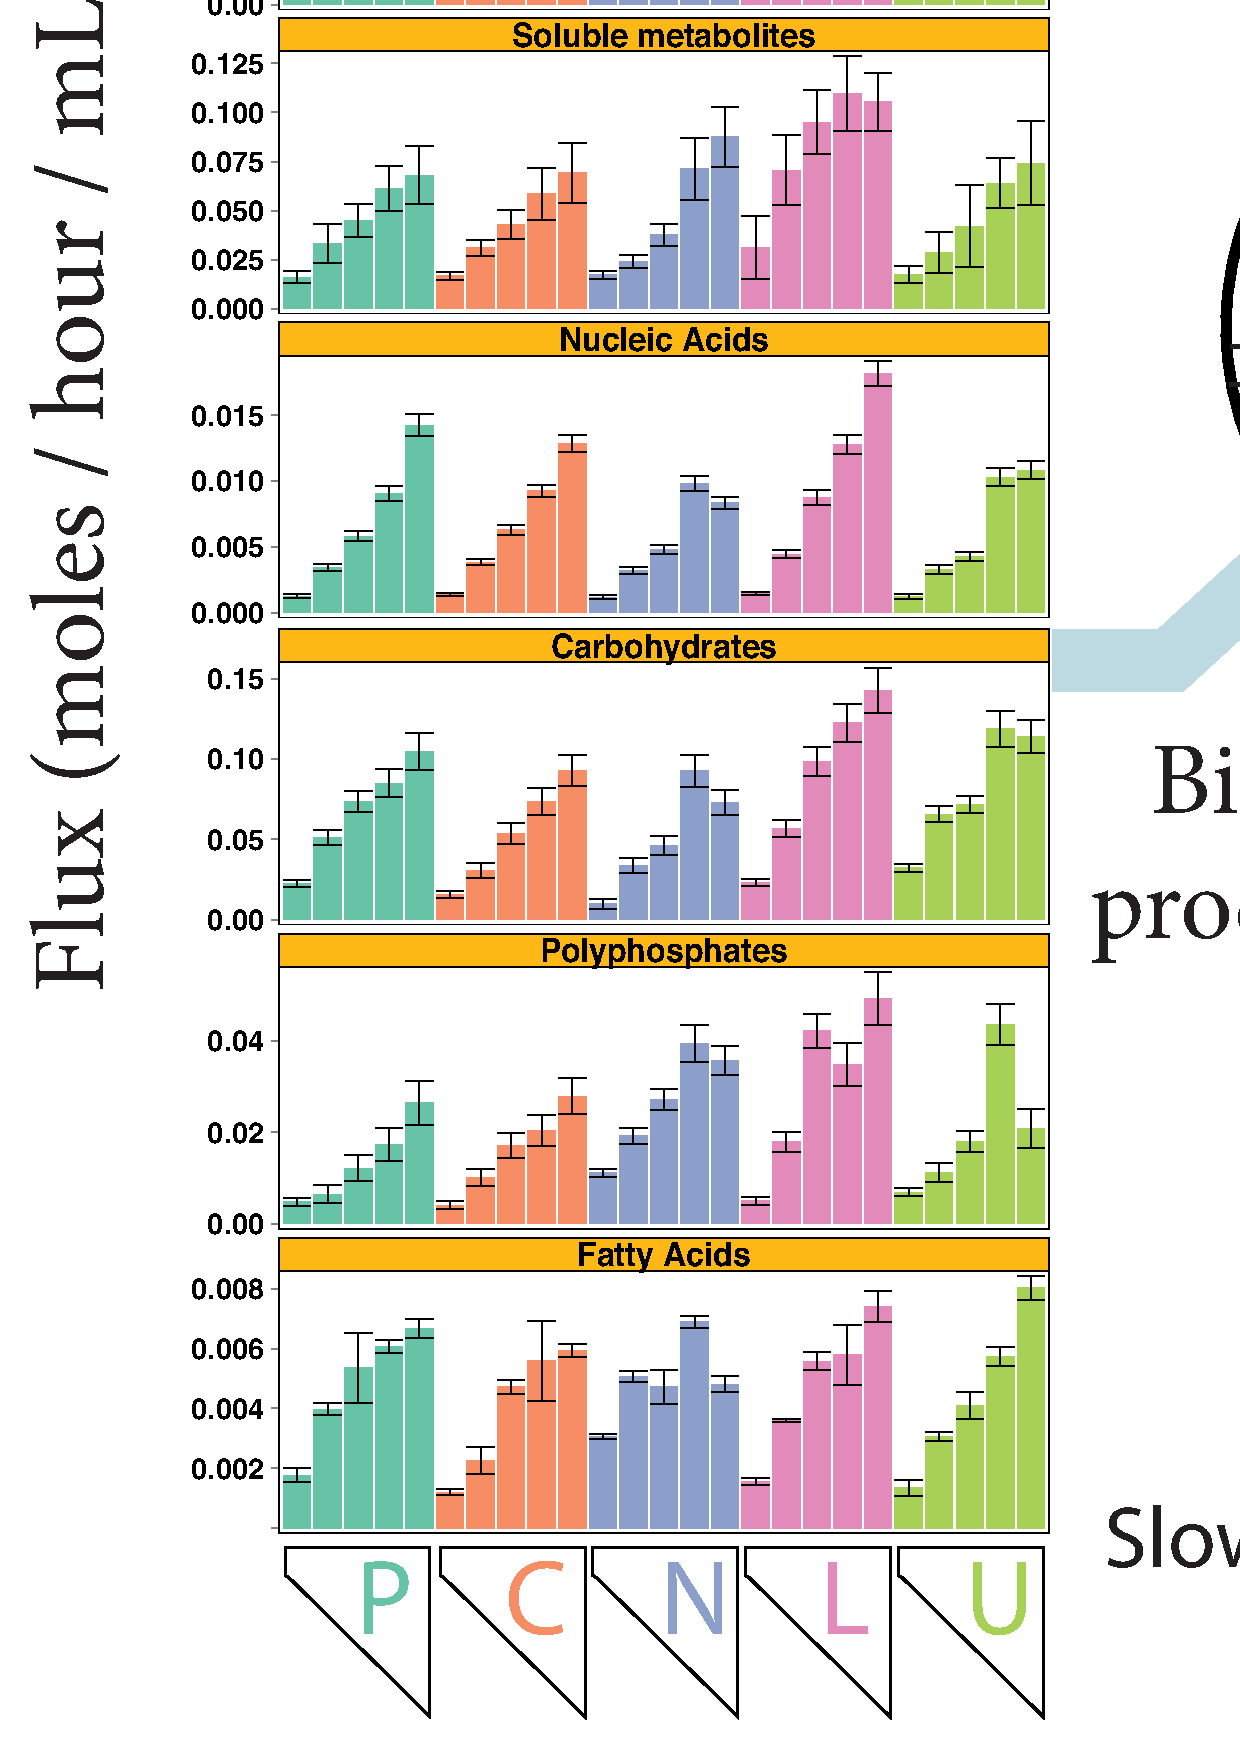
\includegraphics[width = 0.8\textwidth]{Figures/Supplement/boundaryFluxes.pdf}
\caption{Summary of experimentally-determined rates of metabolite uptake, excretion and incorporation into biomass for each chemostat condition. }
\label{fig:boundFlux}
\end{figure}

\begin{figure}[h!]
\includegraphics[width = 0.7\textwidth]{Figures/Supplement/fluxHM.pdf}
\caption{Heatmap summarizing relative flux through 233 reactions across chemostat conditions.  Absolute reactions fluxes were determined independently for each chemostat and to visualize reactions whose flux was correlated, the flux through each reaction was expressed relative to the median absolute flux across all conditions.  Reactions were organized using hierarchical clustering using absolute pearson correlation with average linkage.  Only reactions that were well-constrained based on flux variability analysis are shown.}
\label{fig:fluxHM}
\end{figure}

\begin{figure}[h!]
\includegraphics[width = 1\textwidth]{Figures/Supplement/peptide_RA_reproduce.pdf}
\caption{Nutrient-induced changes in peptide abundance between technical replicates are highly reproducible.  As a representative example, a slow growth nitrogen-limited chemostat (n0.05) is compared to an internal reference slow-growth phosphorous-limited $^{15}$N-labelled chemostat ($^{15}N$-p0.05).  For each of two technical replicates, derived from independent digestion, fractionation and mass spectrometry of a single sample, the relative abundance of unlabelled experimental peptides relative to $^{15}N$-labelled reference peptides is shown.}
\label{fig:proteomicsConsistency}
\end{figure}

\begin{figure}[h!]
\includegraphics[width = 0.7\textwidth]{Figures/Supplement/proteinHM.pdf}
\caption{Heatmap summarizing the variable concentration of 1187 proteins across chemostat conditions. From the ratio of unlabelled sample peptides to matching $^{15}N$-labelled reference peptides, the abundance of each enzyme relative to a common reference was determined.  Across the 25 conditions, protein relative abundances were mean-centered, log-transformed and organized by hierarchical clustering using pearson correlation with average linkage.}
\label{fig:proteinHM}
\end{figure}

%\begin{figure}[h!]
%\includegraphics[width = 1\textwidth]{Figures/Supplement/TPMomicsDesignVarEx.pdf}
%\caption{The relative impact of growth rate and limiting nutrients in driving systematic variation of transcripts, proteins, enzymes and metabolites was tested through comparison of nested regression models.  Proceeding from simpler to more complicated models, the fraction of variation explained across all genes/metabolites explained by the added term indicates its relative impact on abundance.  The order of model progression was: intercept $\rightarrow$ GR + intercept $\rightarrow$ GR + limitation $\rightarrow$ GR * limitation.  Results were robust to whether GR or limitation were added first.}
%\label{fig:TPMomics}
%\end{figure}

\begin{table}[H!]
\centering
\begin{tabular}{l>{\hfill}p{0.5in}>{\hfill}p{0.5in}>{\hfill}p{0.5in}>{\hfill}p{0.5in}>{\hfill}p{0.5in}>{\hfill}p{0.5in}}
 \begin{sideways} \begin{turn}{-90}\textbf{Pathway}\end{turn} \end{sideways} & \begin{sideways} \multilineL{Reactions with\\measured enzymes} \end{sideways} & \begin{sideways} \multilineL{Total pathway\\reactions} \end{sideways} & \begin{sideways} \multilineL{Fraction of reactions\\with measured enzymes} \end{sideways} & \begin{sideways} \multilineL{Measured enzymes} \end{sideways} & \begin{sideways} \multilineL{Total enzymes} \end{sideways} & \begin{sideways} \multilineL{Fraction of\\measured enzymes} \end{sideways} \\ 
  \hline
\multicolumn{1}{l||}{Glycolysis / Gluconeogenesis} &  16 &  16 & 100\% &  17 &  18 & 94\% \\ 
  \multicolumn{1}{l||}{Citrate cycle (TCA cycle)} &  12 &  12 & 100\% &  12 &  12 & 100\% \\ 
  \multicolumn{1}{l||}{Biosynthesis of amino acids} &  73 &  83 & 88\% &  63 &  75 & 84\% \\ 
  \multicolumn{1}{l||}{Purine metabolism} &  37 &  52 & 71\% &  28 &  41 & 68\% \\ 
  \multicolumn{1}{l||}{Pyrimidine metabolism} &  27 &  39 & 69\% &  22 &  31 & 71\% \\ 
  \multicolumn{1}{l||}{All reactions} & 346 & 524 & 66\% & 304 & 510 & 60\% \\ 
   \hline
\end{tabular}
\caption{For major metabolic pathways, the coverage of enzymes measured through proteomics is summarized.  For each pathway, we show both the the fraction of reactions where at least one enzyme was measured, as well as the total fraction of enzymes measured.  Pathway annotation are based on KEGG.} 
\label{protTable}
\end{table}

%\begin{figure}[h!]
%\includegraphics[width = 0.7\textwidth]{Figures/Supplement/enzymes.pdf}
%\caption{Heatmap summarizing the variable concentration of 370 enzymes across chemostat conditions. From the ratio of unlabelled sample peptides to matching $^{15}N$-labelled reference peptides, the abundance of each enzyme relative to a common reference was determined.  Across the 25 conditions, enzyme relative abundances were mean-centered, log-transformed and organized by hierarchical clustering using pearson correlation with average linkage.}
%\label{fig:enzymeHM}
%\end{figure}

\begin{table}[ht]
\centering
\begin{tabular}{|l|l|l|r|}
  \hline
Reaction Name & Regulation & Support & Rank \\ 
  \thickhline
3-phosphoglycerate dehydrogenase & (-) Serine & \textcolor{BurntOrange}{Alternative regulation supported} &  88 \\\hline
\multirow{2}{*}{Acetolactate synthase} & (+) ATP & \textcolor{ForestGreen}{Strongest support} &  15 \\ 
   & (-) Valine & Other GS supported &  55 \\\hline
  Acetylglutamate kinase & (-) Arginine & \textcolor{BurntOrange}{No tested model is adequate} & 108 \\\hline 
  Asparagine synthetase & (-) Asparagine & \textcolor{Cerulean}{No physiological regulation} &  38 \\\hline 
  Aspartate carbamoyltransferase & (-) UTP & \textcolor{BurntOrange}{Alternative regulation supported} & 101 \\\hline 
  \multirow{2}{*}{Aspartokinase} & (-) Homoserine & \textcolor{LimeGreen}{Supported} &  22 \\ 
   & (-) Threonine & \textcolor{ForestGreen}{Strongest support} & 19 \\\hline 
  ATP phosphoribosyltransferase & (-) Histidine & \textcolor{LimeGreen}{Supported} &  78 \\\hline 
  Carbamoyl phosphate synthase & (-) UTP & \textcolor{Cerulean}{No physiological regulation} &  70 \\\hline 
  CTP synthase & (-) CTP & \textcolor{BurntOrange}{No tested model is adequate} &   8 \\\hline 
  \multirow{2}{*}{DAHP synthase} & (-) Phenylalanine & \textcolor{LimeGreen}{Supported} &  23 \\ 
   & (-) Tyrosine & \textcolor{LimeGreen}{Supported} &  15 \\\hline 
  Glutamate 5-kinase & (-) Proline & \textcolor{ForestGreen}{Strongest support} &  14 \\\hline 
  Homocitrate synthase & (-) Lysine & \textcolor{ForestGreen}{Strongest support} &   7 \\\hline 
  Homoserine kinase & (-) Threonine & \textcolor{BurntOrange}{No tested model is adequate} &  82 \\\hline 
  \multirow{3}{*}{Phosphofructokinase} & (+) AMP & \textcolor{BurntOrange}{Alternative regulation supported} & 109 \\ 
   & (-) ATP & \textcolor{BurntOrange}{Alternative regulation supported} &  25 \\ 
   & (+) Fructose 2,6-P$_{2}$ & Not measured &  \\\hline 
  PRPP amidotransferase & (-) AMP & \textcolor{ForestGreen}{Strongest support} &  32 \\\hline 
  \multirow{4}{*}{Pyruvate kinase} & (-) ATP & Other GS supported &  46 \\ 
   & (+) Ammonia & Not measured &  \\ 
   & (-) Citrate & \textcolor{LimeGreen}{Supported} &  15 \\ 
   & (+) Fructose 1,6-P$_{2}$ & \textcolor{LimeGreen}{Supported} &   6 \\ 
   \hline
\end{tabular}
\caption{Support for previously identified regulation.  Previous analysis of 16 reactions in yeast has strongly implicated a role for 24 catalytically important regulators.  22 of these 24 regulatory relationships could be tested using the SLIMER methodology.  For each reaction, an optimal hypothetical activator's or inhibitor's relative abundance trend was found, and each gold-standard regulator's correlation with this optimal regulator was ranked relative to all 109 measured metabolites.}
\label{tab:GS}
\end{table}

\begin{figure}[h!]
\includegraphics[width = 1\textwidth]{Figures/Supplement/HIStimecourse.pdf}
\caption{Inhibition of His1p by histidine is contingent upon the reaction product, phosphoribosyl-ATP.   \textbf{A)} Cumulative flux through HIS1 shows that while reaction rate is initially independent of histidine concentration, as the reaction proceeds the effect of histidine emerges. The cumulative flux at each concentration of hisitidine can be well-explained using a cubic polynomial fit using regression. \textbf{B)} Instantaneous flux, i.e. the derivative of the fitted cumulative flux, was compared to phosphoribosyl-ATP concentration.  Flux decreases as phosphoribosyl-ATP accumulates and the inhibitory effect of histidine increases with phosphoribosyl-ATP concentrations.}
\label{fig:atpprtase}
\end{figure}

\begin{figure}[h!]
\includegraphics[width = 1\textwidth]{Figures/Supplement/OTCaseAla.pdf}
\caption{Alanine is a physiological regulator of ornithine carbamoyltransferase.  \textbf{A)} \textit{In vitro} measurement of the impact of alanine concentration on purified Arg3p indicates that alanine is an allosteric inhibitor with a k$_{i}$ of about 14.8 mM.  \textbf{B)} Physiological concentrations of alanine vary greatly and are around the affinity for Arg3p implying meaningful difference in occupancy and inhibition.  \textbf{C)} Alanine inhibition of OTCase could serve as a way of directing flux into pyrimidine synthesis under high-amino acid conditions that should favor ribosome production.  When pyrimidine needs are met, a paired regulation of ATCase favors flux into Arginine production for nitrogen and carbon storage.}
\label{fig:otcase}
\end{figure}


\begin{figure}[h!]
\includegraphics[width = 0.6\textwidth]{Figures/Supplement/hypoMetAnalysis.pdf}
\caption{Using optimal regulators to investigate the regulation of understudied reactions.  Looking at 10 reactions which each had less than five annotated regulators, we identified both an optimal hypothetical metabolite activator and an inhibitor that resulted in the greatest improvement in fit.  \textbf{A)} Of these 10 reactions, the kinetic fit of four reactions was improved by either an optimal activator or inhibitor relative to Michaelis-Menten kinetics and three of these reactions were significant relative to models containing regulation.  \textbf{B)} For each of the three reactions were an optimal activator or inhibitor was best supported, the metabolites that are most strongly correlated with the optimal regulator were noted as regulatory candidates.}
\label{fig:hypoMet}
\end{figure}

\begin{table}[H!]
Excel file summarizing all supported regulation for each reaction
\caption{}
\label{tab:all_rxn}
\end{table}

\begin{figure}[h!]
\includegraphics[width = 0.9\textwidth]{Figures/Supplement/performanceSummary.pdf}
\caption{Predicted metabolite affinities are consistent with literature reports and reveal different trends in occupancy for substrates, products and regulators. \textbf{A)} Using the best-fit reaction forms, the affinity of substrates and products with measured absolute concentrations were compared to metabolite affinities found in BRENDA.  For 73\% of metabolites, the parameter 95\% CI contains the literature consensus affinity (mean of log$_{10}$ affinities), while for 89\% of metabolites, the 95\% CI overlaps the sampling distribution of literature estimates (mean $\pm 2 \cdot \sigma$(log$_{10}$ affinities). \textbf{B)} Using the best-fit reaction forms, occupancies implied by the MAP estimate of affinities for every measured substrate, product and regulator were compared. The shown violin plot was generated using one occupancy value for each metabolite's affinity for an enzyme in every condition.  To determine if this pattern differed between substrates, products and regulators, for each class, median relative affinity MAP estimates formed an empirical distribution that could be compared to the log-uniform expectation using a KS test (* p $<$ 0.05; *** p $<$ 0.001). The number of metabolite-enzyme affinities used for each class is listed.}
\label{fig:occupancy}
\end{figure}

\begin{figure}[h!]
\includegraphics[width = 0.9\textwidth]{Figures/Supplement/parameterSummary.pdf}
\caption{Predicted reaction thermodynamics are consistent with reported literature. \textbf{A)} Demonstrating parameter estimates using Triose-phosphate isomerase with reversible Michaelis-Menten kinetics as an example.  Affinity parameters are varied relative to the median metabolite concentration and K$_{eq}$ is determined relative to the median reaction quotient (Q), giving the disequilibrium ratio ($\rho = \sfrac{Q}{K_{eq}}$).  The value of each parameter is summarized by the maximum posterior (MAP) estimator and by the 95\% credibility interval (CI).  The lower hinge of the median disequilibrium ratio specifies the minimal permissible disequilbrium needed for approximately correct prediction.  \textbf{B)} Using the best-fit reaction forms, the MAP estimate of median disequilbirium (blue circle) and minimal permissible disequilbirium (black cross-bar) are shown.  To visualize how disequilbirium changes across conditions, the density of reaction quotients for each condition is shown about the minimal permissible disequilbrium; for reactions where the MAP estimate is near the minimal permissible disequilibrium this variation in disequilibrium is kinetically important.  To compare inferred disequilbirium to literature reports, the disequilbrium in fast-growth carbon-limited chemostat (green circle) can be compared to findings from batch-culture.  Looking at glycolysis, we see that this approach accurately predicts that the step with the greatest disequilbirium are phosphofructokinase and pyruvate kinase, while steps that are closer to equilibrium, PGK and TPI are highly reversible.}
\label{fig:paramaterValues}
\end{figure}


%\begin{figure}[h!]
%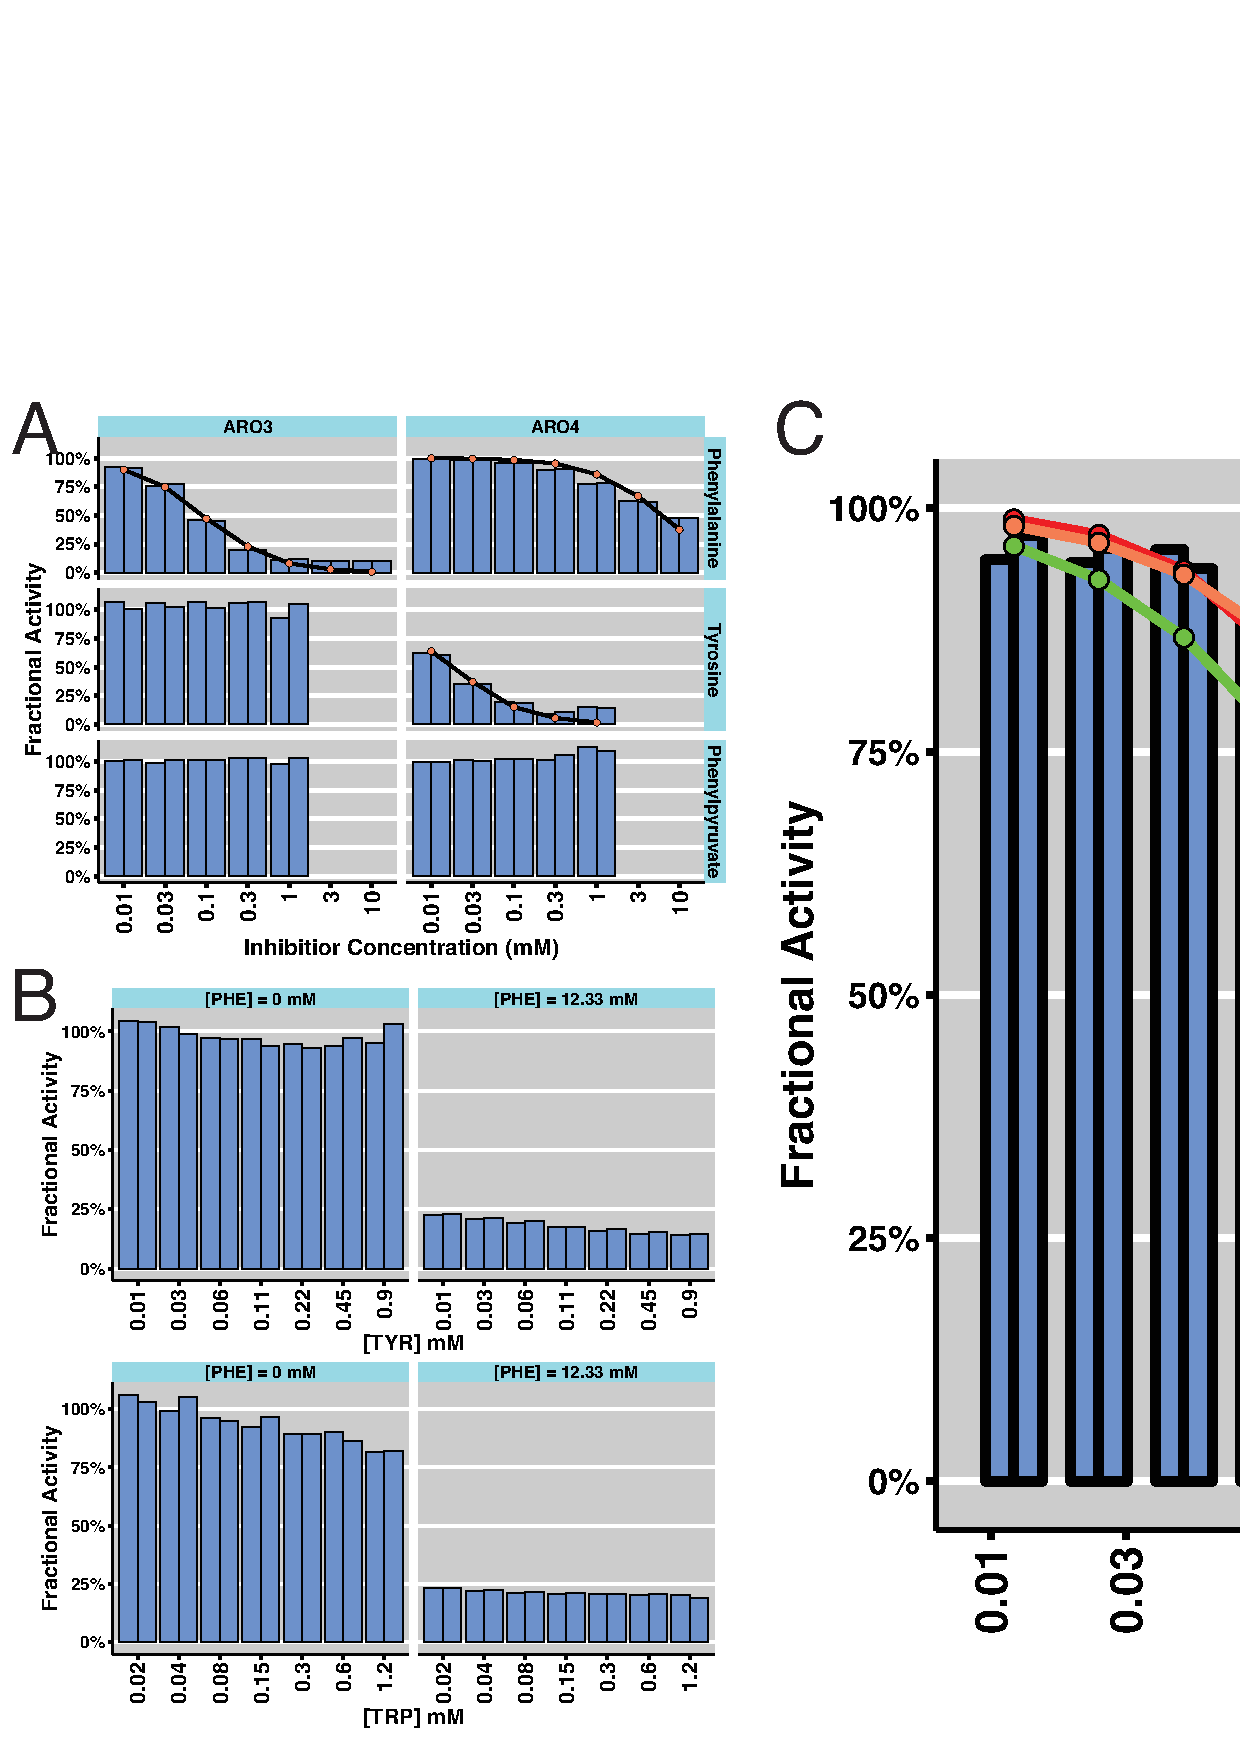
\includegraphics[width = 1\textwidth]{Figures/Supplement/DAHPsummary.pdf}
%\caption{DAHP isoenzymes are strongly regulated through complex isoenzyme-specific inhibition. \textbf{A)} Aro3p is strongly inhibited by phenylalanine, Aro4p is strongly inhibited by tyrosine and weakly inhibited by phenylalanine.  Relative activity at high concentrations of inhibitor is greater than would be expect based on standard uncompetitive inhibition. \textbf{B)} Residual activity of Aro3p that is phenylalanine-insensitive is not abolished through the addition of tyrosine or tryptophan.  \textbf{C)} The \textit{in vitro} kinetics of phenylalanine inhibiting Aro3p can be explained by allowing for constitutive activity and cooperative inhibitor binding.}
%\label{fig:dahp}
%\end{figure}

%\begin{figure}[h!]
%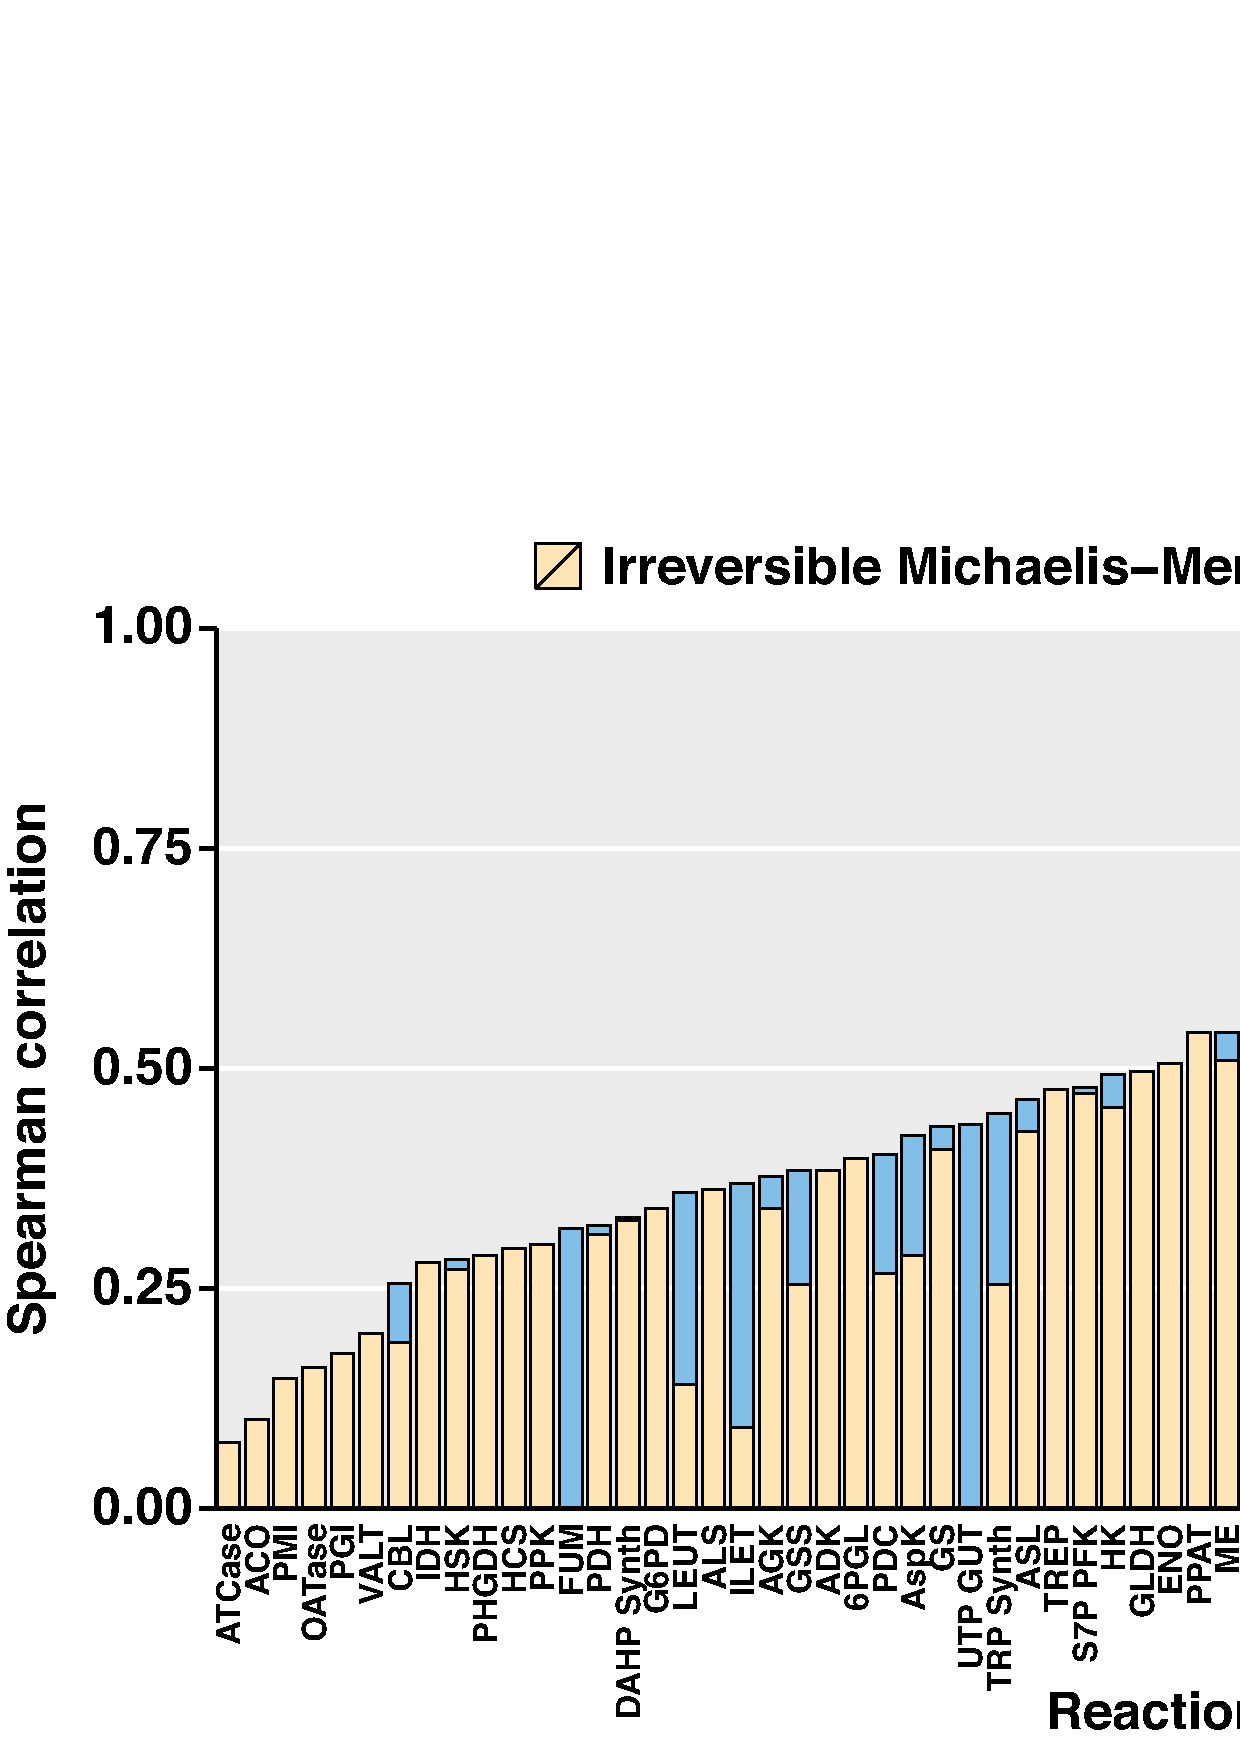
\includegraphics[width = 1\textwidth]{Figures/Supplement/reversibilityFitImprovement.pdf}
%\caption{Metabolism-wide summary of the role of reaction reversibility in driving net flux. For each of 55 reactions, the spearman correlation between measured flux and Michaelis-Menten kinetics with and without reversibility was assessed.}
%\label{fig:reversibilityFit}
%\end{figure}

\begin{figure}[h!]
\includegraphics[width = 1\textwidth]{Figures/Supplement/metabolicLeverageBar.pdf}
\caption{Summary of substrates, products, enzymes and regulator metabolic leverage.  The metabolic leverage of each reaction is shown grouping species into four classes: substrates, products, enzymes and regulators. If multiple species fall into a single class then their contributions were summed. The median metabolic leverage of each class across natural limitations (carbon-, nitrogen- or phosphorous-limitation) based on the MAP estimates of kinetic parameters was used and renormalized such that metabolic leverages summed to one for each reaction.}
\label{fig:MLbar}
\end{figure}

\begin{figure}[h!]
\includegraphics[width = 1\textwidth]{Figures/Supplement/MLsupp.pdf}
\caption{WRITE}
\label{fig:MLpathways}
\end{figure}

\begin{figure}[h!]
\includegraphics[width = 1\textwidth]{Figures/Supplement/MCA.pdf}
\caption{Two metabolic control analysis based models of glycolysis were created, one contains the feed-forward activation of pyruvate kinase by fructose 1,6-bisphosphate and an alternative model lacked this regulation. Each model contains five enzymatic steps, phosphofructokinase (PFK), aldolase (ALD), glyceraldehyde dehydrogenase (GAPDH), phosphoglycerate kinase (PGK) and pyruvate kinase (PyK) and four intervening metabolite pools, fructose 1,6-bisphosphate (FBP), glyceraldehyde 3-phosphate (GA3P), 1,3-bisphospho-D-glycerate (1,3BPG) and 3-phosphoglycerate (3-PG). The distribution of flux control coefficients and metabolite concentration control coefficients are shown for each markov sample using the slow-growth nitrogen-limited chemostat as a representative condition.  In both models, phosphofructokinase has a flux control coefficient of near one, while comparing the models with and without FBP activation of pyruvate kinase indicates that this regulation alters concentration control coefficients. In this model pyruvate kinase activity is greatly determined by FBP concentrations while the concentration of PEP is relatively unimportant, thus when aldolase activity increases accumulation of metaoblites upstream of pyruvate kinase would be expected.}
\label{fig:MCA}
\end{figure}



\end{document} 
